\documentclass{article}
\usepackage{graphicx}
\usepackage{latexsym}
\usepackage[french]{babel}
\usepackage[utf8]{inputenc}
\usepackage[T1]{fontenc}
\usepackage{listings}

\title{Rapport du projet C++ : Lancer de rayons}
\author{Mathieu \textsc{Mari} \and Xavier \textsc{Montillet}}

\begin{document}

\title
\tableofcontents
	

\section{Introduction}
Dans ce nouveau projet, nous nous sommes intéressé à la technique du lancer de rayons et nous l'avons implémenter en C++.
Cette technique permet de générer des images 3D à partir de la déscription des objets présent dans la scène ainsi que de la position de la caméra. Elle a son utilité dans les logiciels d'images de synthèse, la création de jeux vidéos, la simulation numérique\dots  	

\section{Implémentation en C++}
	\subsection{Principe général}
	\paragraph{}		
Afin de générer l'image 3D d'une scène, il faut deja définir quels sont les objets qui composent la scène, c'est dire définir quel est leur type (sphère, plan, \dots), quelle est leur position, leur couleur, leur texture\dots. Ensuite, il faut choisir la posistion des sources lumineuses puis leur couleur, leur intensité\dots Enfin, il faut positionner la caméra qui observe la scène. Pour cela, on choisit un point qui sera la position de l'objectif, puis la position de l'ecran sur lequel l'image sera projetée.

	\paragraph{}
		Fabriquer une image, c'est calculer pour chaque pixel sa couleur. Dans cette optique, le principe de la technique du lancer de rayons consiste à créer une demi-droite ayant pour origine l'objectif de la caméra et passant par le un pixel de l'écran. On regarde quel objet de la scène est intersecté en premier par la demi-droite. On calcule ensuite la couleur du pixel en regardant combien de sources éclairent le point d'intersection entre la demi-droite et l'objet, quel est la couleur de l'objet et des sources, est-ce qu'il y a reflection, refraction, transparence\dots

		\subsection{Les différentes classes utilisées}

Afin de représenter les différents éléments qui seront nécessaires à la technique du lancer de rayons et leur dépendance mutuelle, nous allons utiliser les classes C++.

\subsubsection{Dépendances des classes}
Le schéma de dépendance des classes est le suivant :
	\begin{center}
    		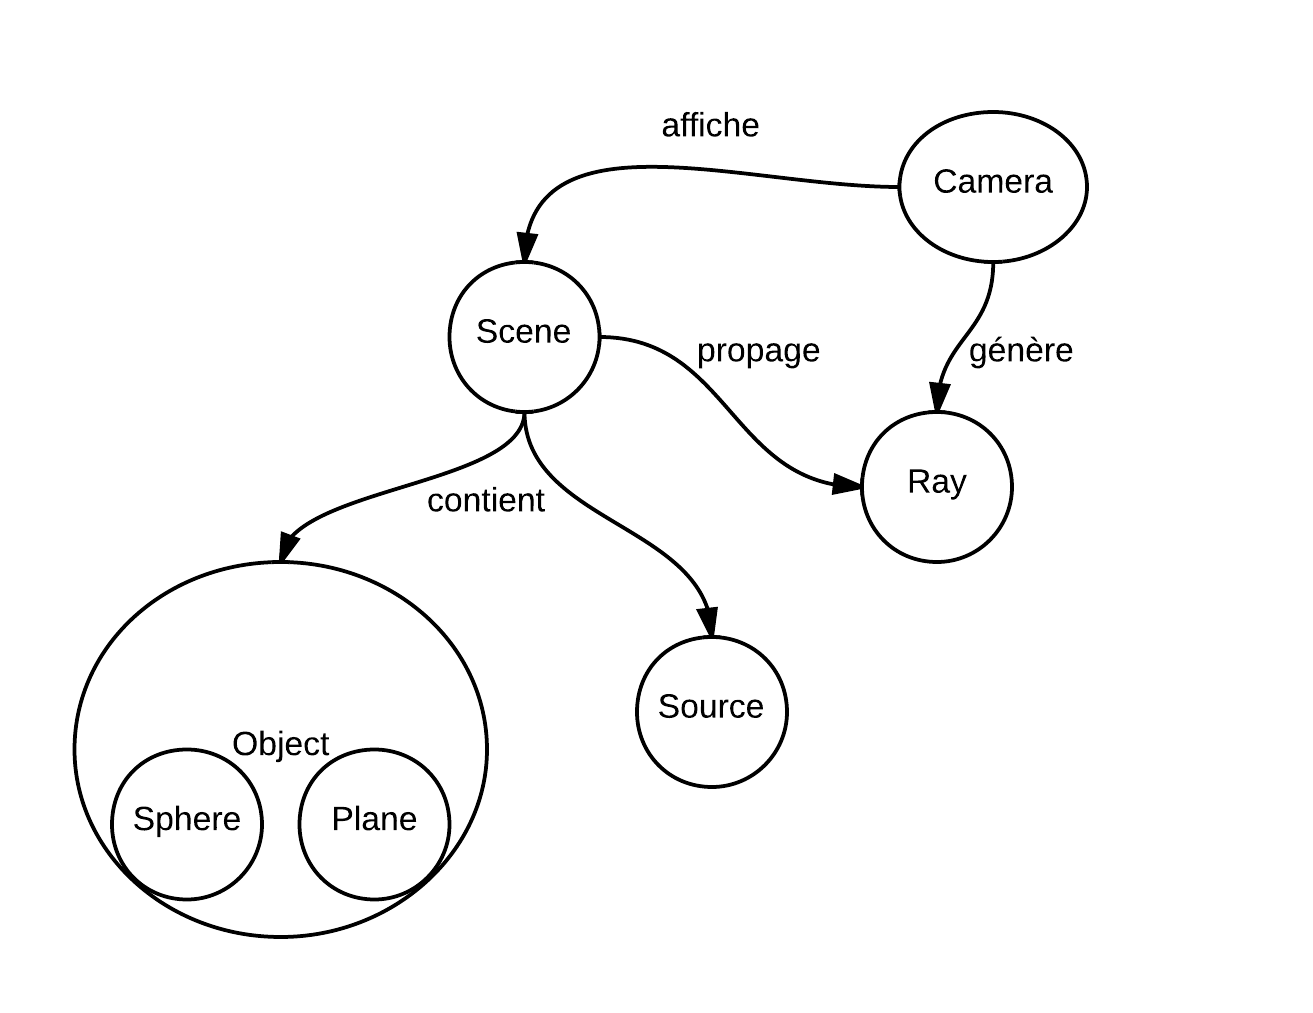
\includegraphics[height = 7cm]{schema.png}
  		\end{center}

	\begin{itemize}
\item La classe \emph{Scene} est la classe principale. Elle contient des objets de la classe \emph{Object} qui contient elle-même deux sous-classes : \emph{Sphere} et \emph{Plane}. 
\item La classe \emph{Scene} contient également des sources lumineuses de la classe \emph{Source}.
\item La caméra, représentée par la classe \emph{Camera} est indépendante de la classe \emph{Scene} car il nous semblait raisonnable que la caméra soit indépendante le la scène. En effet, la scène n'a pas besoin de savoir où se situe la caméra : c'est la caméra qui observe la scène! 

\end{itemize}
Toutes ces classes interfèrent entre elles grâce à des rayons de la classe \emph{Ray} : la caméra fabrique des rayons qui vont se propager dans la scène. 



D'autres classes nous sont utiles dans la réalisation de l'algorithme de lancer de rayons.

\subsubsection{La classe \emph{Light}}
Cette classe permet de représenter un rayon lumineux. Elle possède trois attributs : une composante \emph{red}, une composante \emph{green}, et une composante \emph{blue}.
La différence avec la classe \emph{Color} est que les composantes ne sont pas comprisent entre $0$ et $255$ mais entre $0$ et $+\infty$.
Ceci permet de représenter de façon implicite l'intensité d'une lumière, (on peut imaginer prendre le max des composante par exemple). Ceci permet d'additionner des lumières en additionnant simplement composante par composante, sans avoir à se préocuper de faire un barycentre avec différents coefficients. 


Nous avons codé une fonction permettant de transformer une lumière en une couleur (l'image renvoyée à la fin ne connait que des couleurs ayant des composantes comprises entre $0$ et $255$. Pour cela nous composons les composantes par la fonction $x \rightarrow 255\th(x)$. 

\subsubsection{La classe \emph{Texture}}
	La couleur d'un pixel dépend de la texture de l'objet visé. En effet, l'effet visuel ne sera pas le même suivant si l'objet est brillant, mate, transparent\dots La classe \emph{Texture} permet donc de représenter ces différentes caractéristiques. Cette classe est essentielle si nous ne voulons pas à chaque fois redéfinir les méthodes de la classe \emph{Object}. 


  

	


\end{document}
